\documentclass[12pt,titlepage,a4paper]{article}
\usepackage[a4paper, total={6.5 in, 8 in}]{geometry}
\usepackage{graphicx} % Required for inserting images
\usepackage{amsmath}
\usepackage{times}
\pagestyle{plain}% this will add page nuneber under
\graphicspath{ {images/} }
\usepackage{array,url,kantlipsum}
\newcommand{\Mark}[1]{\textsuperscript{#1}}
\usepackage[font=footnotesize]{caption}
\usepackage{float}
\usepackage{xcolor}
\usepackage{titlesec}
\usepackage{setspace}

\begin{document}

\title{University of Toronto \\ CIV 102 Bridge Design Delivery 1}
\author{Jingfei Liu, Stella Yuan, Xuanhao Lu}
\date{November 13th, 2023}
\maketitle


\section{Shear Force Diagram(SFD)\&Bending Moment Diagram(BMD)}
    The following FBD, SFD, and BMD is obtained by hand calculation and verified and drawn by matlab script.
    \begin{figure}[H]
        \centering
        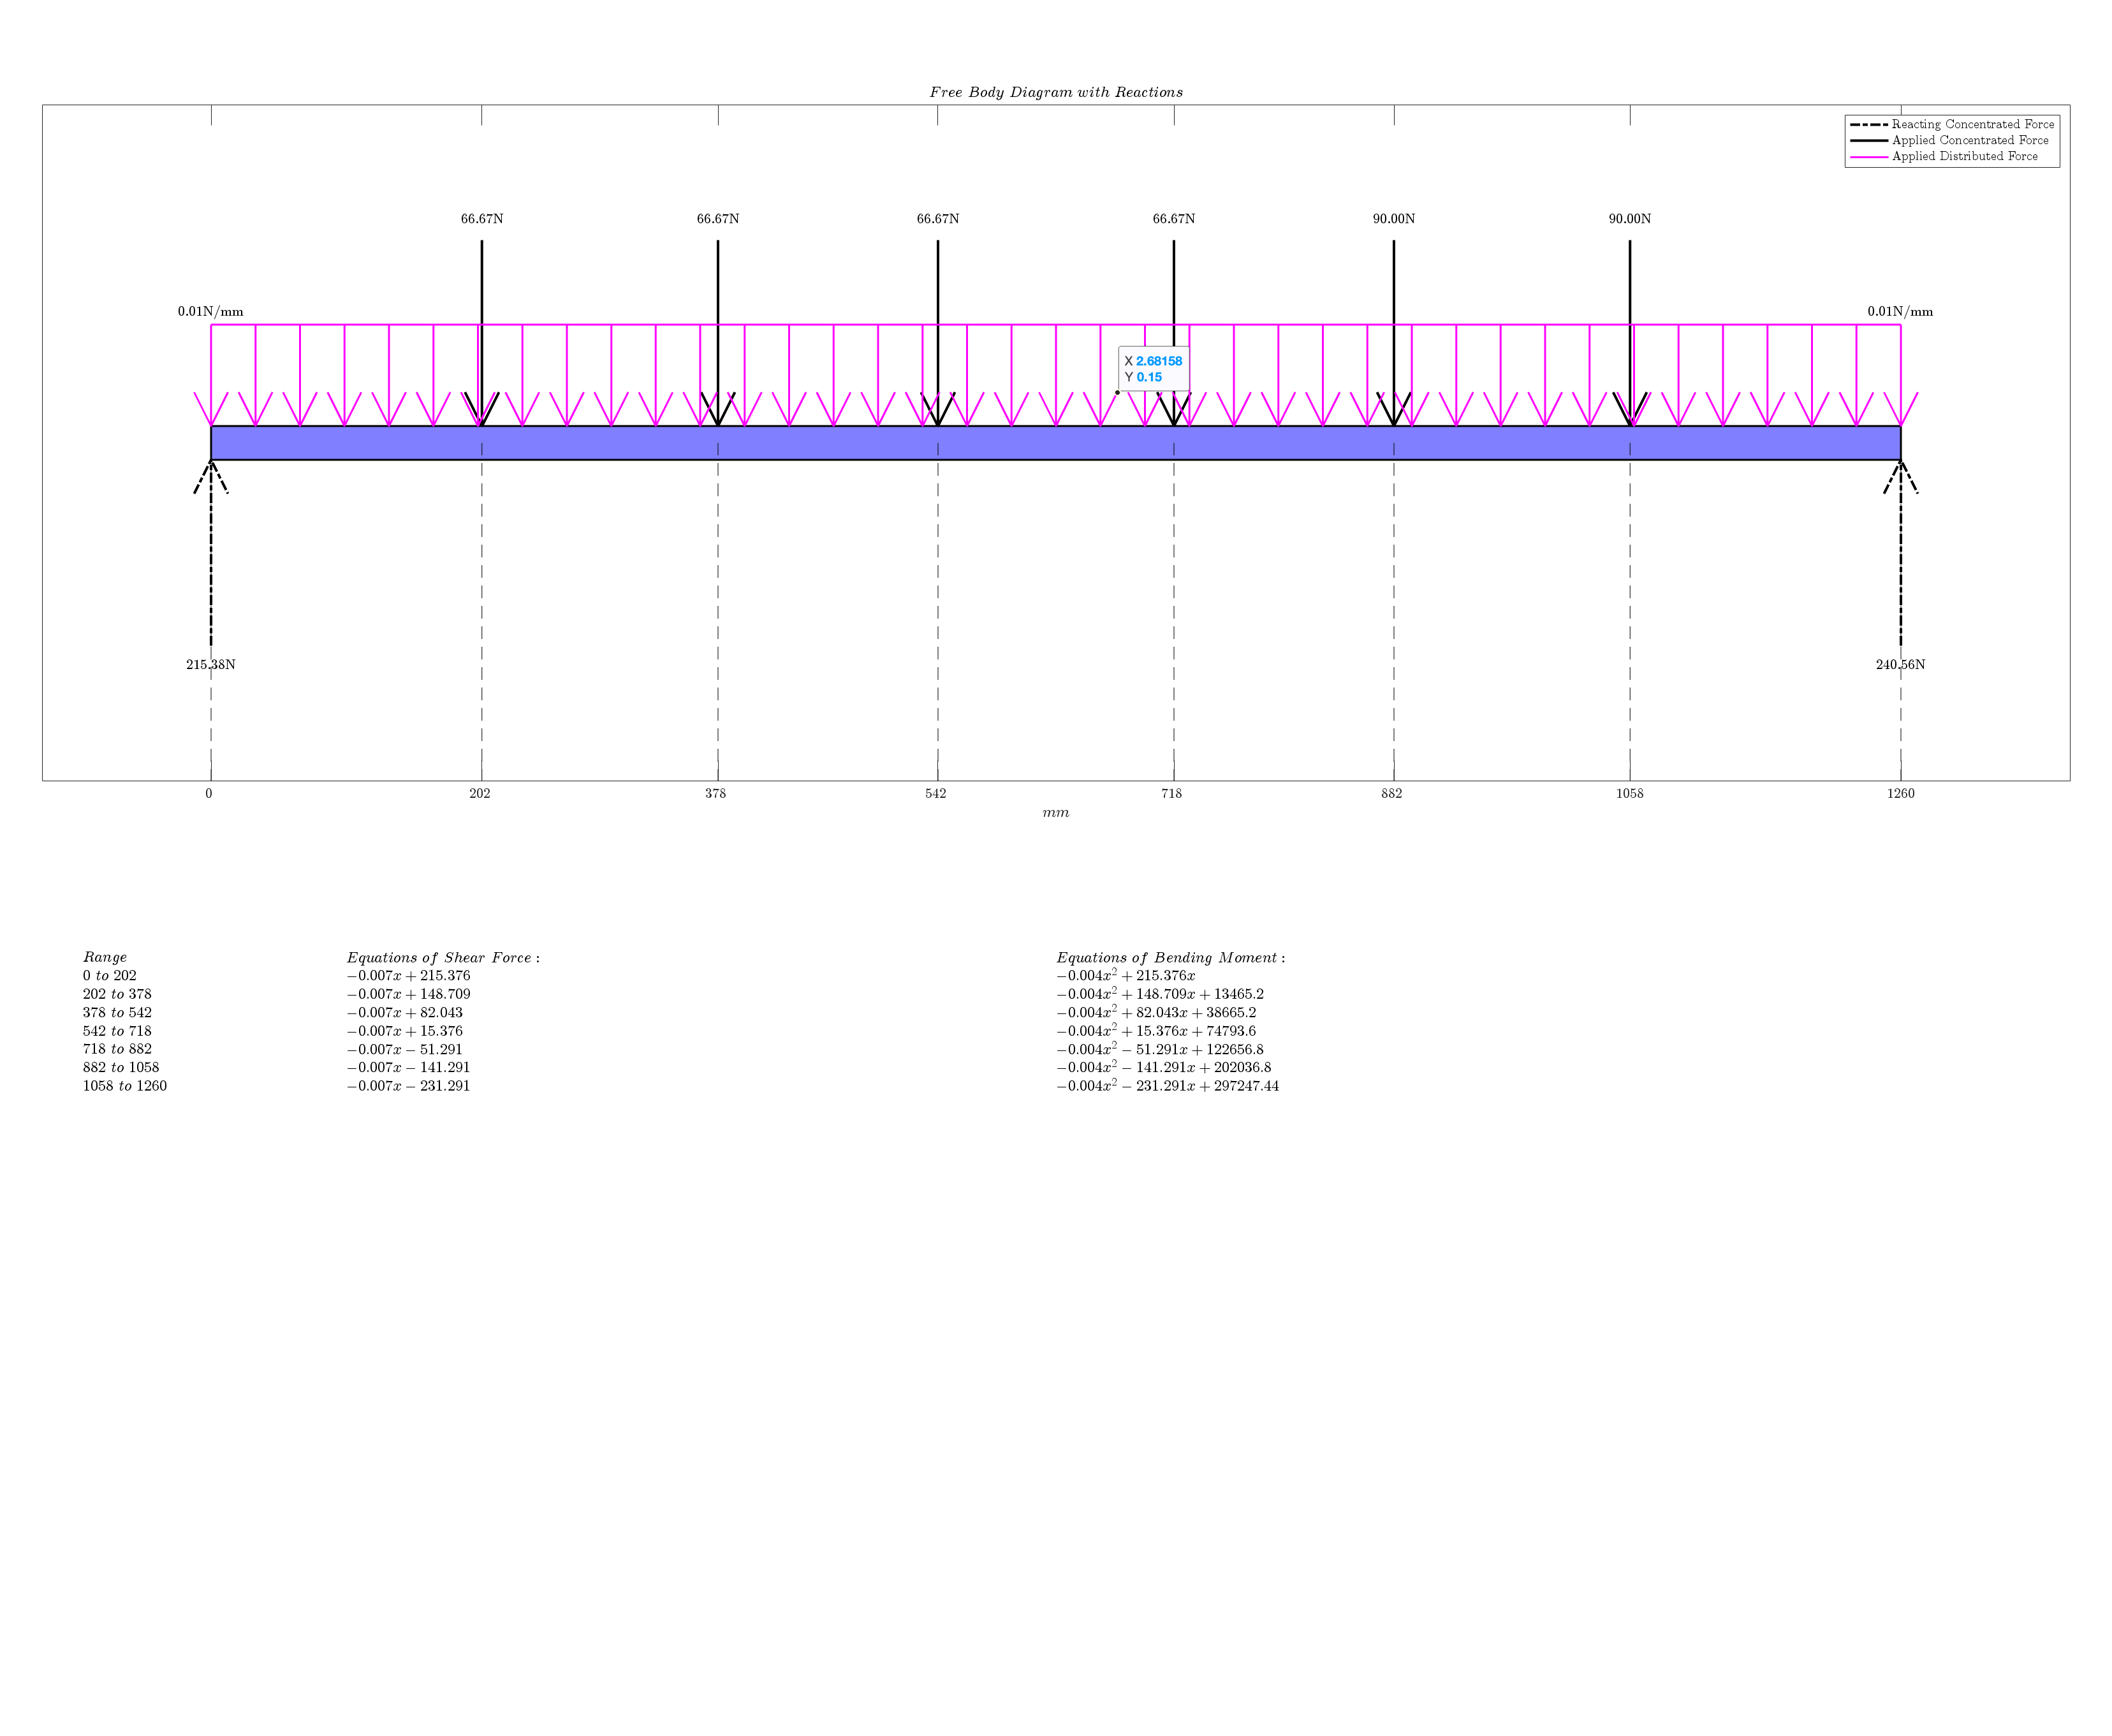
\includegraphics[width=16cm]{Delivery_1_FBD.png}
        \caption*{\textbf{Figure 1.1:} This is the FBD for the base case of load condition 2}
        \label{fig:enter-label}
    \end{figure}
    \begin{figure}[H]
        \centering
        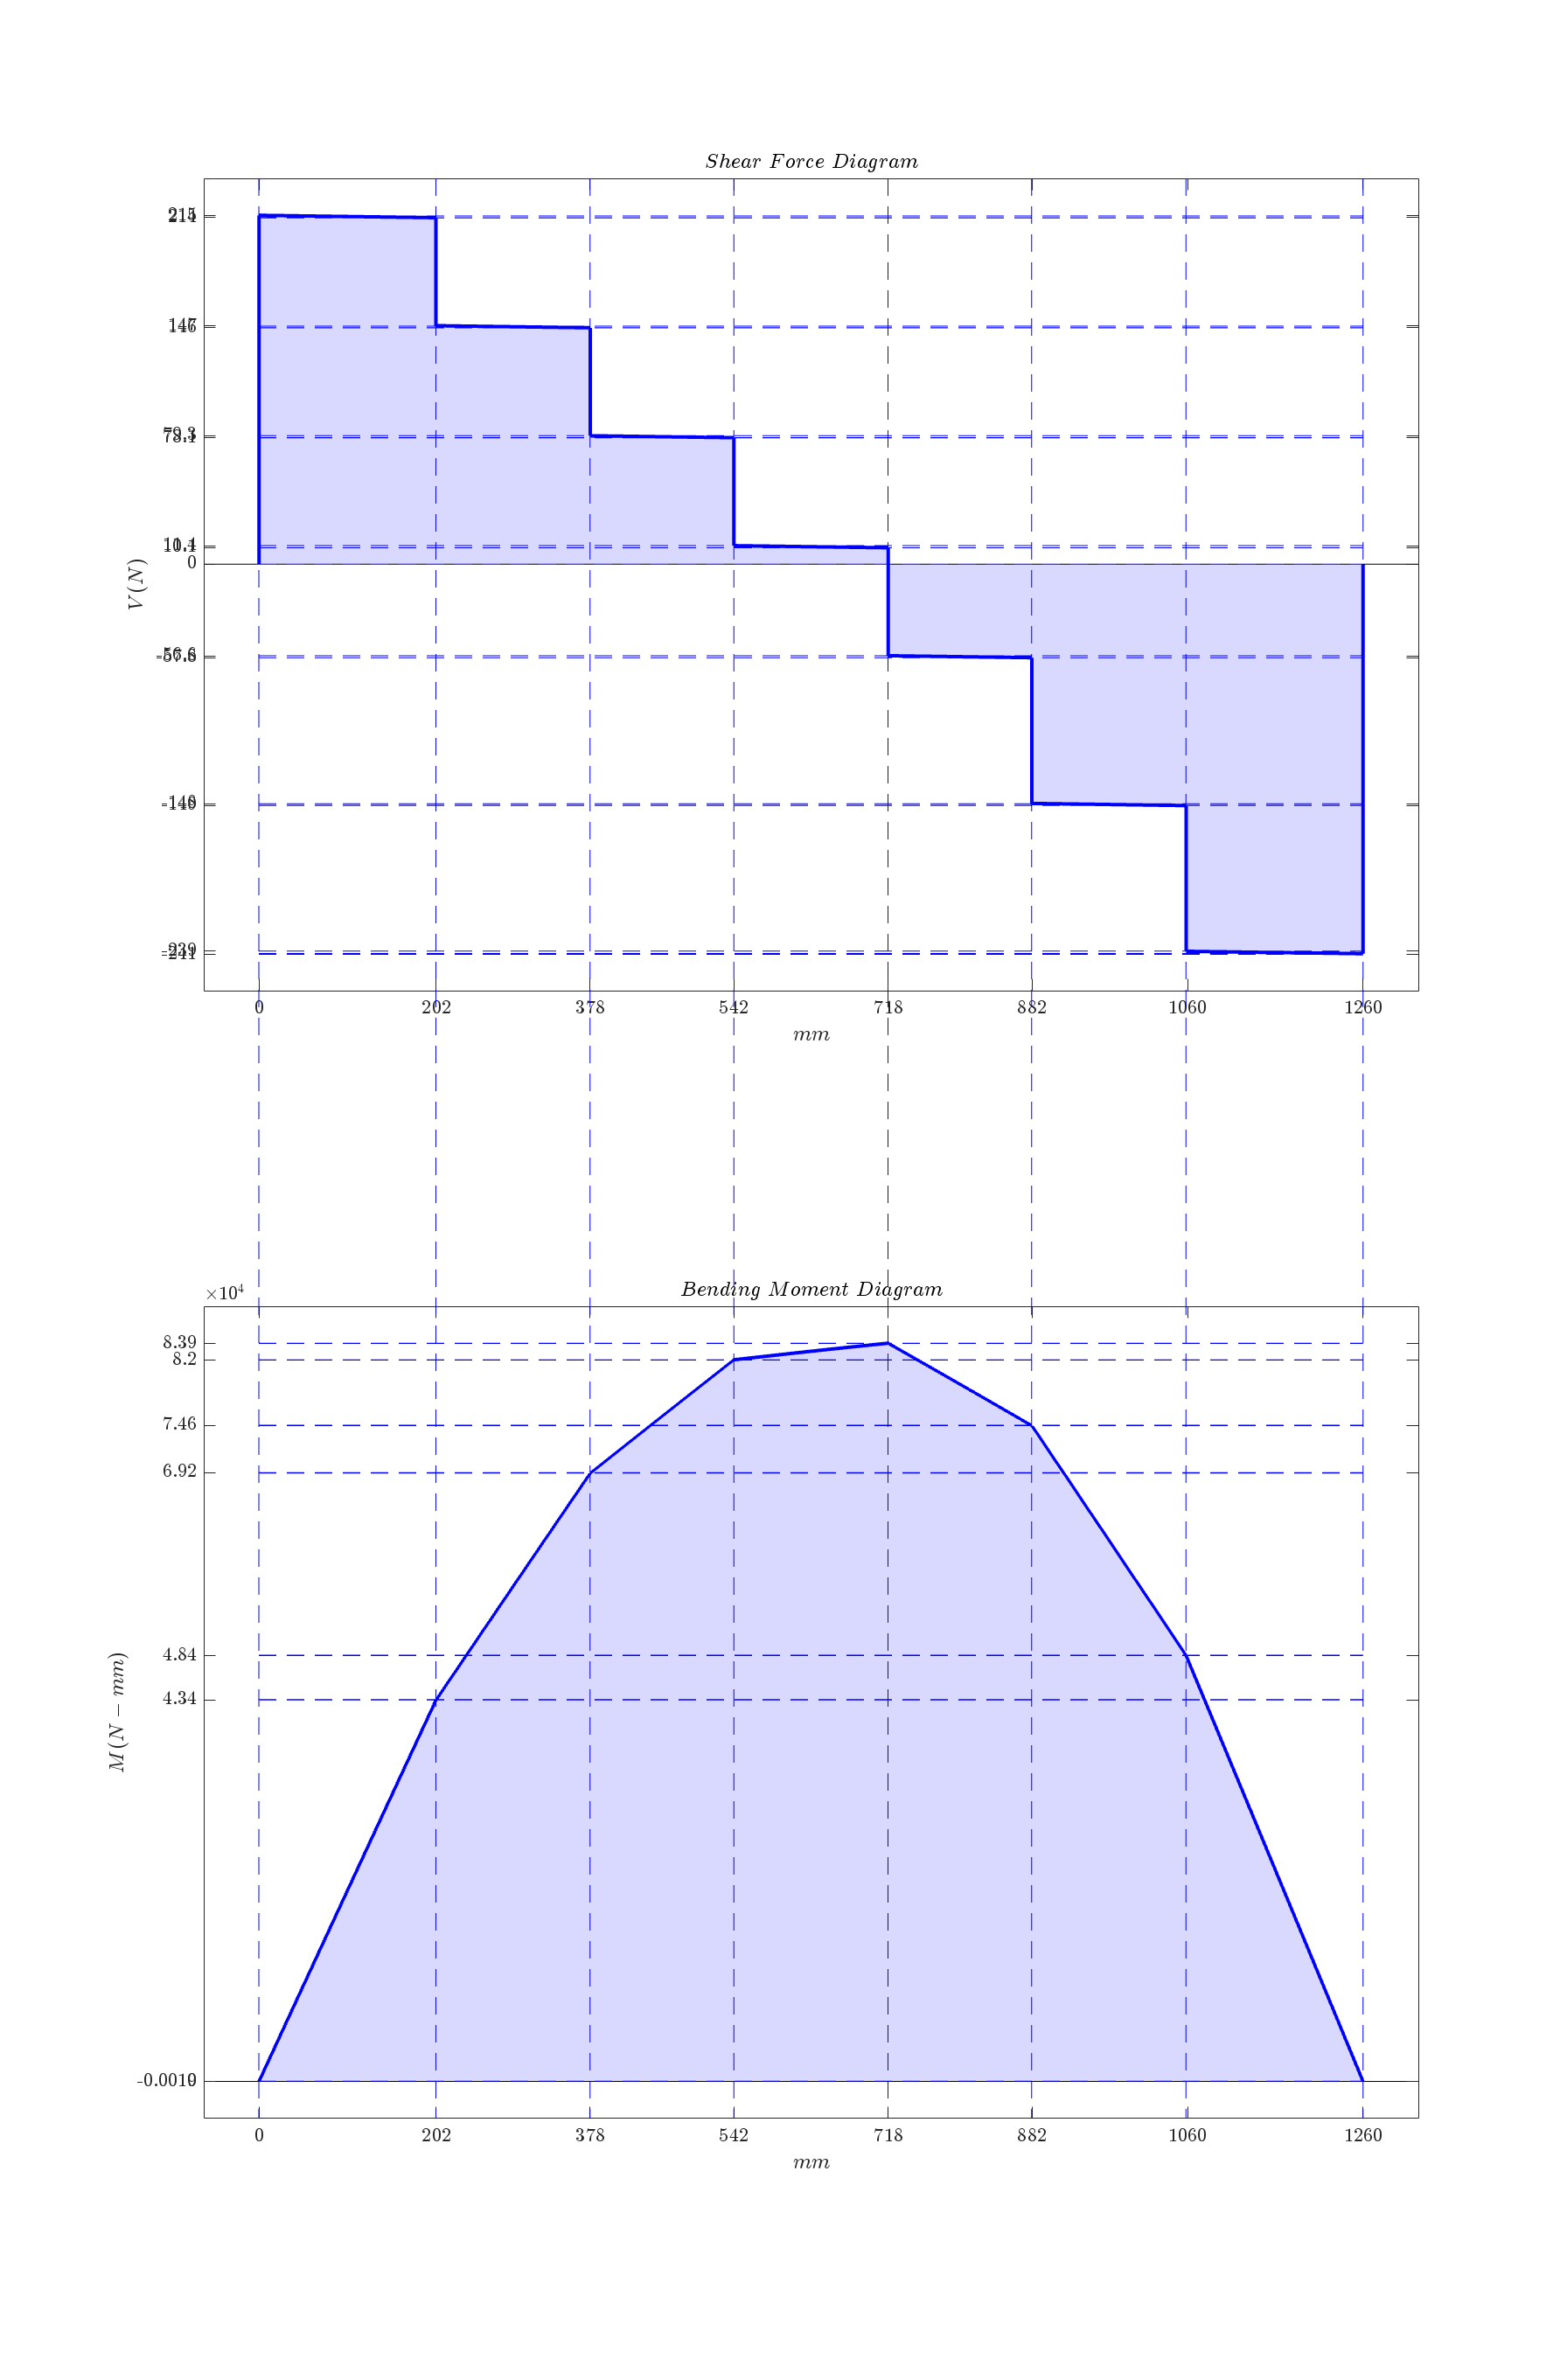
\includegraphics[width=13cm]{Delivery_1_SFD&FBD.png}
        \caption*{\textbf{Figure 1.2:} This is the SFD and the BMD for the base load of condition 2}
        \label{fig:enter-label}
    \end{figure}



    \section{FOS}
        The following results are obtained from calculations done by hand and verfied by Excel. 
        The max monments are obtained from the max value of BMD. The equation used is
        \begin{equation}
            \sigma = \frac{My}{I}
        \end{equation}
        \begin{figure}[H]
            \centering
            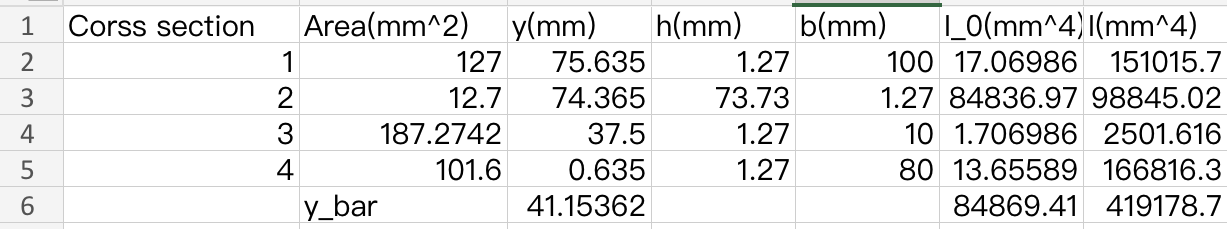
\includegraphics[width=13cm]{m_and_centorid.png}
            \caption*{\textbf{Figure 2.1:} This is the data calcualted for FOS obtained from excel}
            \label{fig:enter-label}
        \end{figure}
        \begin{spacing}{1.5}
        The maximum moment is $8.39\times10^4 N*mm$. \\The distance from the top of the beam to the centorid is 
        $y_{top} = 76.27mm - 40.15m = 36.12mm$. The maximum flexural tension is thus $\sigma_{max, top} = \frac{(8.39\times10^4 N*mm)
        (36.12mm)}{419178.6627mm^4} = 7.23Mpa$. \\The distance from the bottom of the beam to the centorid is 
        $y_{bottom} = \bar{y} = 40.15mm$. 
        \\The maximum flexural compression is thus $\sigma_{max, bottom} = \frac{(8.39\times10^4 N*mm)
        (40.15mm)}{419178.6627mm^4} = 8.04Mpa$. 
        \\The FOS for flexural tension is $FOS_{tension} = \frac{\sigma_{max}}{\sigma}$, which is then $FOS_{tension} = \frac{30Mpa}{7.23Mpa} = 4.15$.
        \\The FOS for flexural compression is $FOS_{compression} = \frac{\sigma_{max}}{\sigma}$, which is then $FOS_{compression} = \frac{6Mpa}{7.23Mpa} = 0.830$.
        \end{spacing}





























\end{document}